\subsection{Comparison of Ordinary MPC and NMPC}
In this section, the Non-linear MPC is tested. The files for the simulation is handed out from the Professor in the course.
\begin{figure}[H]
    \centering
    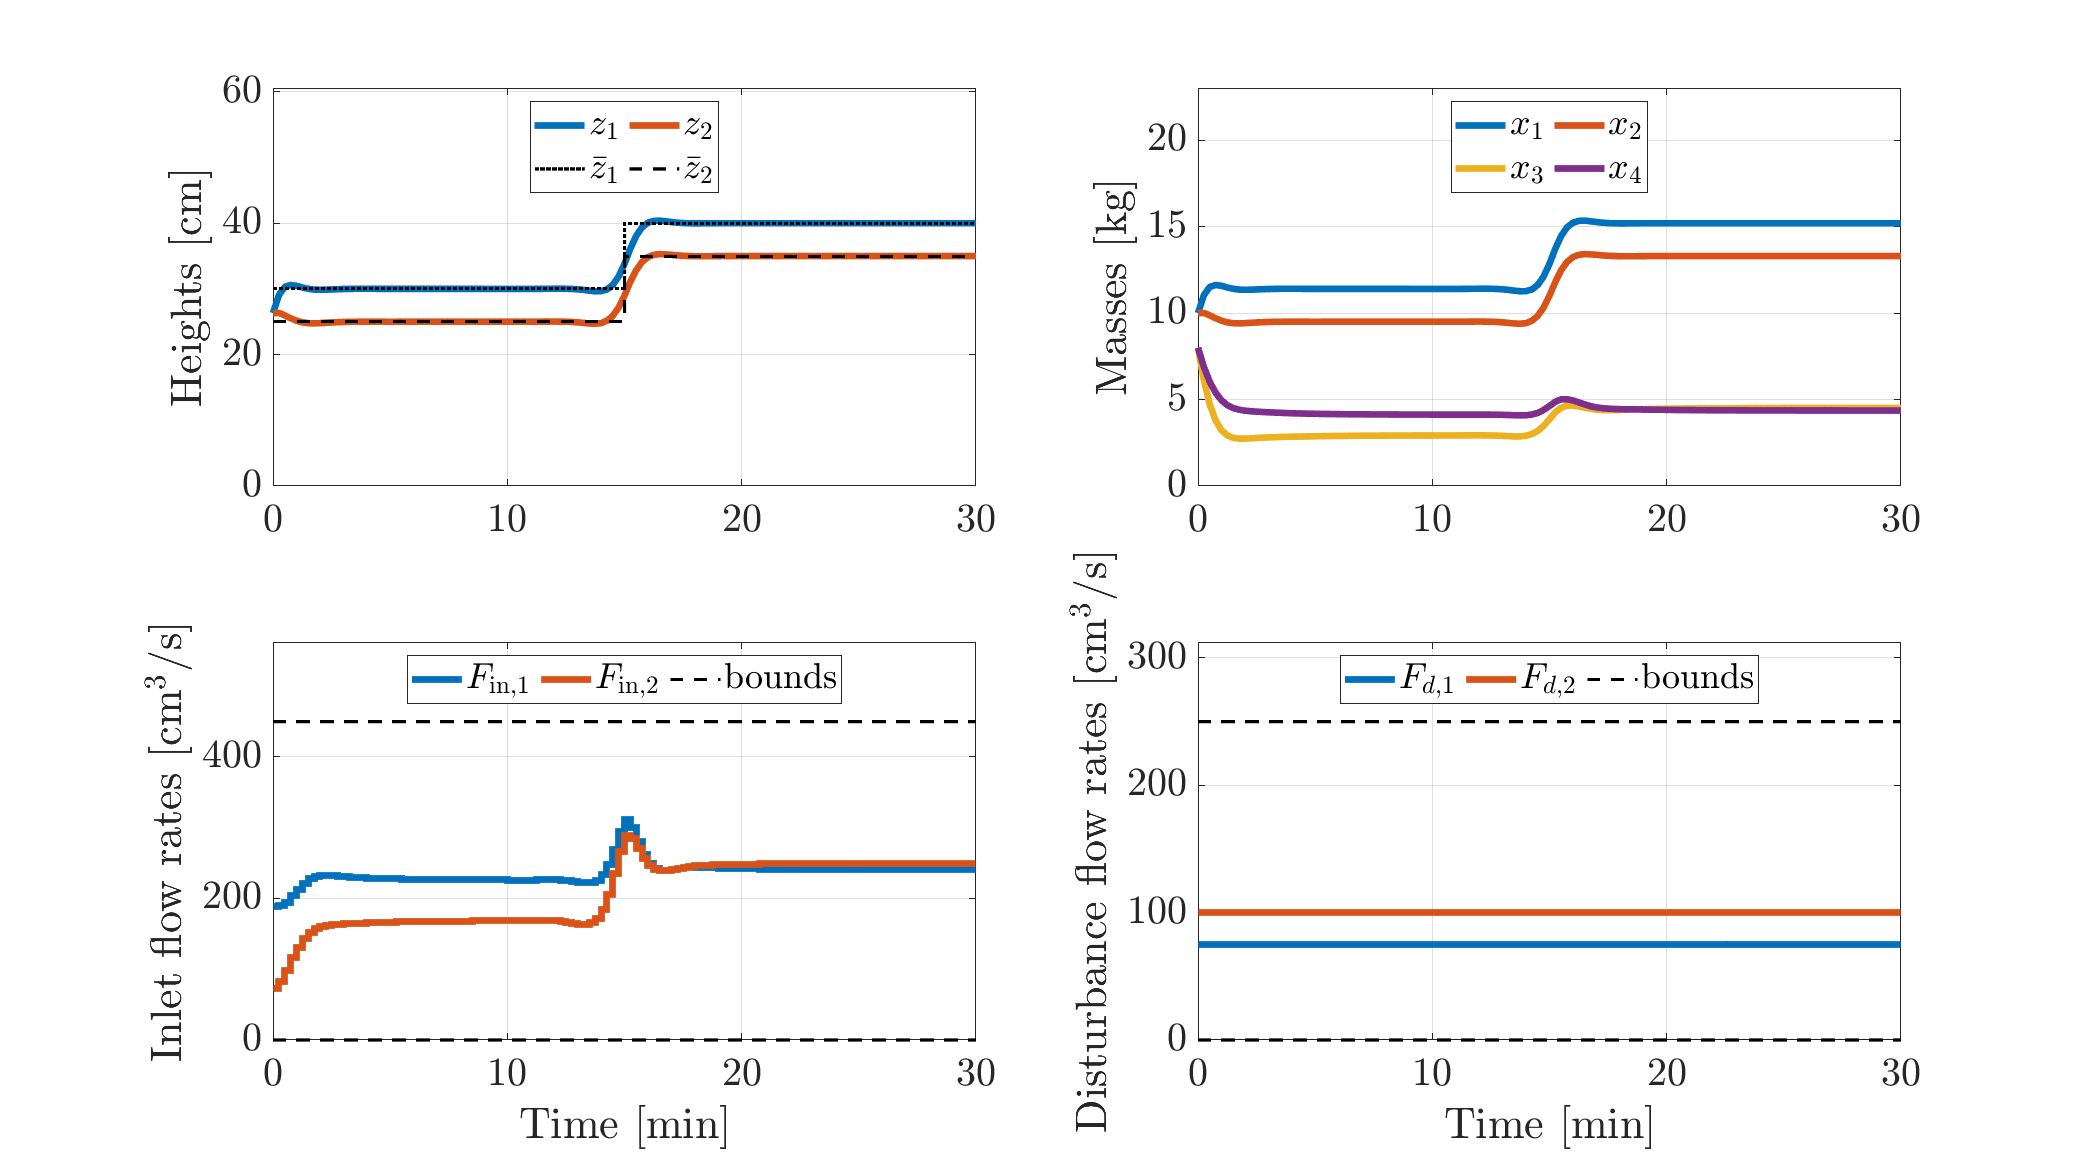
\includegraphics[width=1\textwidth]{Figures/Pr11.5_NonLin_MPC.png}
    \caption{Non-linear MPC - Simulation}
    %\label{fig:Kalman_stoc_state_step}
\end{figure}
It was previously determined that when the unconstrained \textit{MPC} was tested on the non-linear system the deviation from the linearization point was influencing the performance due to non-linearities. As expected, a \textit{NMCP} takes the non-linearities into acocunt thus a better performance is achieved. 